% !TEX TS-program = pdflatex
% !TEX encoding = UTF-8 Unicode
% !BIB TS-program = bibtex
%
% Bayesian station-level Soft Mobility Index (IMD) for French
% bike-sharing systems.
% Authors: R. Foss\'e & G. Pallares (CESI LINEACT, 2025--2026).
%
\documentclass[11pt,a4paper]{article}

% --- Encoding & language ------------------------------------------------
\usepackage[T1]{fontenc}
\usepackage[utf8]{inputenc}
\usepackage{lmodern}
\usepackage[margin=2.5cm]{geometry}
\usepackage{microtype}
\usepackage{csquotes}

% --- Mathematics --------------------------------------------------------
\usepackage{amssymb,amsmath,amstext}

% --- Figures, tables, lists --------------------------------------------
\usepackage{graphicx}
\graphicspath{{figures/}{experiments/outputs/}}
\usepackage{booktabs}
\usepackage{array}
\usepackage{float}
\usepackage{caption}
\captionsetup{font=small,labelfont=bf,labelsep=period}
\usepackage{enumitem}
\setlist{topsep=2pt,itemsep=2pt,parsep=0pt}
\usepackage{url}

% --- Citations ----------------------------------------------------------
\usepackage[authoryear,round]{natbib}
\bibliographystyle{elsarticle-harv}

% --- Hyperlinks ---------------------------------------------------------
\usepackage{xcolor}
\usepackage[colorlinks=true,
            linkcolor=black, citecolor=black, urlcolor=blue!50!black,
            breaklinks=true]{hyperref}

% --- Author block -------------------------------------------------------
\usepackage{authblk}
\renewcommand\Authfont{\normalsize}
\renewcommand\Affilfont{\small\itshape}
\setlength{\affilsep}{0.6em}

% --- Convenience macros -------------------------------------------------
\usepackage{xspace}
\newcommand{\IMD}{\mathrm{IMD}}
\newcommand{\IES}{\mathrm{IES}}
\DeclareMathOperator*{\argmax}{arg\,max}

% =========================================================================
\title{A Bayesian station-level Soft Mobility Index for the audited
       French bike-sharing panel}

\author[1]{Rohan Foss\'e\thanks{Corresponding author. E-mail:
            \texttt{rohan.fosse@gmail.com}.}}
\author[1]{Ga\"el Pallares}
\affil[1]{CESI LINEACT, BikeShare-ICT research programme,
          Montpellier, France}
\date{}

\begin{document}
\maketitle

% =========================================================================
\begin{abstract}
\noindent
French monitoring of bike-sharing performance relies on
volumetric metrics (station count, fleet size, capacity per
inhabitant) that we show fail to predict the cycling
environments cyclists actually experience. We define the
\emph{Soft Mobility Index} (IMD) as a three-component Bayesian
composite -- multimodality, cycling-infrastructure continuity,
topography -- computed at the station level on the
$46\,139$-station audited Gold Standard inventory of
\citet{Fosse2026gold}. The Bayesian formulation places a softmax
prior on the simplex weights, a Gaussian observation model on
the two behavioural reference series (FUB Cycling Barometer
2023, EMP 2019), and recovers the joint posterior on weights and
observation parameters via Metropolis--Hastings. Each station
inherits an IMD posterior distribution; city-level summaries are
the means of the station posteriors and inherit a credible
interval rather than a point estimate.

On the French panel of 59 dock-based urban areas, the posterior
on the multimodality weight $w_M$ is centred at $0.82$
($95\,\%$ CrI $[0.70, 0.89]$) and dominates the other components
in every posterior draw ($P(w_M \text{ dominates}) = 1.00$). The
indicator is therefore empirically a \emph{multimodality index
with infrastructure and topography refinements}. Both reference
slopes are credibly positive: $\beta_{\text{FUB}} = +0.55$
($[+0.28, +0.83]$), $\beta_{\text{EMP}} = +0.69$
($[+0.48, +0.90]$). The Spearman correlation between the
posterior-median IMD and median household income per consumption
unit is $\rho_{\mathrm{Sp}} = +0.04$ ($p = 0.76$): cycling
quality is statistically independent of local income.
Strasbourg, Montpellier and Paris lead the panel; Strasbourg's
posterior-median IMD ($20.5$, CrI $[16.0, 30.0]$) is more than
seven times the score of the median-ranked city in the panel.

The Bayesian framework natively quantifies three sources of
uncertainty that point-estimate composite indicators conflate:
(i) the weights, via the posterior on the simplex; (ii) the
station sampling within a city, via the per-draw aggregation of
station IMDs; (iii) the measurement noise, via the Gaussian
observation model. We document a feed-level data-quality
anomaly (A6) on the GTFS layer of the Gold Standard pipeline
that affects six panel cities; the IMD posterior absorbs the
A6 uncertainty through wider per-city credible intervals on the
affected cities.

All code, data products and posterior draws are released openly
under the FAIR principles.

\smallskip
\noindent\textbf{Keywords:} bike-sharing systems; composite
indicators; Bayesian inference; Metropolis-Hastings; multimodal
accessibility; General Bikeshare Feed Specification;
station-level; France.
\end{abstract}

% =========================================================================
\section{Introduction}
\label{sec:introduction}
% =========================================================================

Cycling is a structural component of French urban mobility
policy. The 2023--2027 National Cycling and Active Mobility Plan
commits roughly EUR\,250 million per year of public investment
in cycling infrastructure and targets a near-tripling of the
cycling modal share between 2024 and 2030. Yet the indicators
that inform the operational steering of this investment are
overwhelmingly \emph{volumetric}: number of bike-sharing stations
per inhabitant, fleet size, capacity. The volumetric prior
implicit in this monitoring is that abundant supply generates
usage. The empirical record contradicts the prior in France:
Strasbourg (39 stations) outranks Paris (1\,507) on every
behavioural cycling outcome we can measure; medium-sized cities
with tight multimodal integration outperform metropolises with
larger fleets.

The contribution of this paper is a context-aware composite
indicator that supersedes the volumetric prior, computed at the
station level rather than the city level, and reported in a
Bayesian form that propagates the three uncertainties currently
hidden by point-estimate composites: the weights of the
constituent components, the within-city sampling of stations,
and the measurement noise. Specifically, we

\begin{itemize}
\item define the Soft Mobility Index (IMD, French \emph{Indice
de Mobilit\'e Douce}) as a three-component composite of
multimodality, cycling-infrastructure continuity and topography,
computed at the station level;
\item formulate the IMD as a Bayesian inference problem with a
softmax prior on the simplex weights and a Gaussian observation
model on two independent behavioural references (the FUB Cycling
Barometer 2023 and the EMP 2019 mobility survey), and sample the
joint posterior via Metropolis--Hastings;
\item propagate the posterior on the weights through the
station-level component matrix to obtain an IMD posterior at
each station and, by station-mean aggregation, at each city;
\item apply the resulting indicator to the
$46\,139$-station Gold Standard panel of \citet{Fosse2026gold}
and report rankings with credible intervals, the relationship
to local income, and the within-city heterogeneity that
city-level point estimates hide.
\end{itemize}

The research questions are:
\begin{itemize}
\item[Q1.] How should a composite indicator of cycling-environment
quality be specified so that it propagates the natural
uncertainties of its calibration and its data inputs?
\item[Q2.] On a national panel of dock-based bike-sharing systems
in France, which of multimodality, cycling-infrastructure
continuity and topography contributes most to the calibrated
composite, and with what credibility?
\item[Q3.] Does the resulting indicator falsify the volumetric
and affluence priors implicit in current policy communications?
\item[Q4.] What does the within-city heterogeneity of the
indicator imply for the granularity at which French
cycling-environment monitoring should operate?
\end{itemize}

Section~\ref{sec:related} situates the contribution.
Section~\ref{sec:data} documents the data inputs and the
upstream Gold Standard pipeline.
Section~\ref{sec:methods} formalises the IMD as a Bayesian
station-level model.
Section~\ref{sec:results} reports the posterior on the weights
and on each city's IMD.
Section~\ref{sec:application} applies the indicator to the
volumetric and affluence priors and to within-city heterogeneity.
Section~\ref{sec:discussion} discusses policy implications and
limitations.
Section~\ref{sec:conclusion} concludes.

% =========================================================================
\section{Related work}
\label{sec:related}
% =========================================================================

\paragraph{Composite indicators and Bayesian inference.}
The methodological foundation for composite indicators is the
\citet{OECD2008} handbook, which formalises the canonical
sequence of normalisation, weighting and aggregation. Weights
are typically elicited normatively, through statistically guided
methods such as CRITIC \citep{Diakoulaki1995} or principal
component analysis \citep{Nardo2005}, or by supervised
optimisation against an external reference
\citep{Saisana2005, OECD2008}. Bayesian alternatives are
comparatively rare in the composite-indicator literature
despite the natural fit: a posterior on weights propagates
naturally to a posterior on the indicator, and the credible
intervals replace the point-estimate plus separate
sensitivity-analysis tradition with a single coherent
uncertainty statement. \citet{Saltelli2008} and
\citet{Saisana2005} explicitly recommend reporting weight
uncertainty alongside point estimates.

\paragraph{Cycling-environment determinants.}
The empirical literature converges on a set of cycling-environment
determinants that motivate our three components. Dedicated
cycling infrastructure is the most established correlate of
cycling adoption \citep{Pucher2010, Heinen2010, Buehler2012,
Garrard2008, Schoner2014}. Multimodal integration with heavy
public transit amplifies cycling at the trip
\citep{Saberi2018}, station-pair \citep{FaghihImani2014} and
infrastructure-design \citep{Martens2007, ElGeneidy2016} levels.
Relief is a documented barrier \citep{Parkin2008, Rietveld2004,
Heinen2010} partly offset by electric-assist bicycles
\citep{Fishman2016, Eren2020}. Safety is consistently identified
as a barrier \citep{Garrard2012, Reynolds2009, Pucher2010,
Aldred2016}, but objective crash-density measures suffer from
cyclist-exposure confounding \citep{Reynolds2009, Schepers2014}
that we discuss in Section~\ref{sec:methods}.

\paragraph{French bike-sharing audits.}
The companion Gold Standard paper \citep{Fosse2026gold} audits
the 122 French GBFS systems, formalises a five-class anomaly
taxonomy (A1--A5) and a six-step purging protocol, and releases
the certified \texttt{46\,139}-station catalogue we consume in
the present work. Module~4 of that pipeline ingests national
GTFS feeds for the multimodality component; we report a
feed-level completeness gap (A6) on three regional GTFS
feeds in Section~\ref{sec:val-a6} and propose a triangulation
patch that the next Gold Standard release should ingest.

% =========================================================================
\section{Data}
\label{sec:data}
% =========================================================================

\subsection{The Gold Standard inventory}

We consume the Gold Standard release of \citet{Fosse2026gold}
as a frozen input: 46\,139 certified stations across 122
bike-sharing systems and 57 urban areas in metropolitan France.
The companion paper documents the five-class GBFS anomaly
taxonomy (A1 out-of-domain inclusion, A2 placeholder capacity,
A3 structural over-capacity, A4 geospatial error, A5 out of
perimeter) and the six-step purging protocol that produces the
certified output. We restrict to the \emph{dock-based} subset
(stations of type \texttt{docked\_bike}) since the
three-component IMD presupposes a fixed station footprint; the
analytical panel comprises 59 urban areas with at least five
certified dock-based stations.

\subsection{Component inputs}

The three component inputs are computed within a 300\,m buffer
around each station, following the last-mile literature
\citep{ElGeneidy2016, Saberi2018}.
\begin{itemize}
\item \emph{Multimodality} ($M$) -- the count of heavy
public-transport stops within 300\,m, sourced from the
national GTFS aggregation on \texttt{transport.data.gouv.fr}.
\item \emph{Cycling-infrastructure continuity} ($I$) -- the
share of road centerline length within 300\,m that carries a
dedicated cycling facility, sourced from OpenStreetMap.
\item \emph{Topography} ($T$) -- the standard deviation of
altitude at the centre and four cardinal offsets at 300\,m
distance from the station, sourced from SRTM 30\,m.
\end{itemize}
A fourth axis, cyclist safety, is constructed by the Gold
Standard pipeline from the BAAC accident registry but we do not
include it in the composite for two empirical reasons: the
exposure-confounding documented by \citet{Reynolds2009} and
\citet{Schepers2014} -- cities with more cyclists record more
crashes -- and the absence of credible discriminative
information that survives the calibration in
Section~\ref{sec:methods}. The safety axis is reported
separately in the companion repository.

\subsection{Behavioural references}

Two independent behavioural references calibrate the
indicator. The \emph{FUB Cycling Barometer 2023} provides
subjective cyclist-perception scores at city level for 32 panel
cities; the \emph{French National Mobility Survey 2018--2019}
(EMP 2019, INSEE/SDES) provides the official bike modal share
by urban area for 44 panel cities. We use both references
because they target distinct constructs (perception vs
behaviour) and impose distinct constraints on the calibration.

\subsection{A note on GTFS completeness}
\label{sec:val-a6}

The national GTFS aggregation used by Module~4 of the Gold
Standard pipeline under-covers the tramway and metro networks
of three French metropolises (Lyon, Marseille, Lille) and three
medium-sized cities (Valenciennes, Clermont-Ferrand, Pau,
Tarbes) by more than an order of magnitude when triangulated
against the equivalent OpenStreetMap heavy-transit tag set. We
name this feed-level anomaly class \emph{A6} as a complement to
the station-level A1--A5 taxonomy of \citet{Fosse2026gold} and
recommend a triangulated $M = \max(C_M^{\mathrm{GTFS}},
C_M^{\mathrm{OSM}})$ patch for the next Gold Standard release.
In the present paper the A6 cities are handled \emph{within the
Bayesian framework}: their per-station component values are
ingested as published and the additional uncertainty due to A6
propagates naturally into a wider posterior credible interval
on the affected cities' IMD (Section~\ref{sec:results-ranking}).

% =========================================================================
\section{Methods: the Bayesian station-level IMD}
\label{sec:methods}
% =========================================================================

\subsection{Component normalisation}

Each raw component is normalised on the dock-based station
panel to $[0, 1]$ by Min--Max scaling:
$C_{k,s} = (c_{k,s} - \min_t c_{k,t}) / (\max_t c_{k,t} -
\min_t c_{k,t})$ for $k \in \{M, I, T\}$ and $s$ indexing
stations. For topography we invert the sign after normalisation
so that a high $C_T$ corresponds to a flat (cycling-friendly)
environment.

\subsection{The composite}

The IMD of station $s$ is a convex combination of the three
normalised components:
\begin{equation}
\IMD_s \;=\; w_M\,C_{M,s} + w_I\,C_{I,s} + w_T\,C_{T,s},
\qquad
\sum_k w_k = 1,\;\; w_k \geq w_{\min}.
\label{eq:imd-station}
\end{equation}
The simplex constraint with floor $w_{\min} = 0.05$ prevents
any component from being zeroed out by the calibration.
City-level IMD is the panel-mean of station IMDs in the city,
$\IMD_i = |\mathcal{S}_i|^{-1} \sum_{s \in \mathcal{S}_i}
\IMD_s$, with $\mathcal{S}_i$ the set of dock-based stations
in urban area $i$.

\subsection{Bayesian formulation}

We parameterise the weights through a softmax pre-image
$\mathbf{z} \in \mathbb{R}^{3}$:
\begin{equation}
\mathbf{w}(\mathbf{z}) = w_{\min}\mathbf{1}
                       + (1 - 3 w_{\min})\,
                         \mathrm{softmax}(\mathbf{z}),
\label{eq:softmax}
\end{equation}
which guarantees that the simplex and floor constraints are
satisfied for any $\mathbf{z}$.

The calibration links the IMD to two behavioural references
through a Gaussian observation model. Let $\tilde{y}_i$ denote
the standardised value of a reference series ($\tilde{y}_i =
(y_i - \bar y) / s_y$, computed separately for FUB and EMP).
For each reference $y \in \{\text{FUB}, \text{EMP}\}$ and each
city $i$ in the matched sub-panel:
\begin{equation}
\tilde{y}_i \;\sim\;
   \mathcal{N}\!\bigl(\alpha_y + \beta_y \cdot
                       \widetilde{\IMD}_i,\; \sigma_y^{2}\bigr),
\label{eq:likelihood}
\end{equation}
where $\widetilde{\IMD}_i$ is the standardised city-level IMD
implied by the current $\mathbf{w}$ and the fixed component
matrix.

The priors are
\begin{align}
\mathbf{z}  &\sim \mathcal{N}(\mathbf{0},\, \sigma_w^{2}\,\mathbf{I}),
                  &\sigma_w &= 1.5,\\
\alpha_y, \beta_y &\sim \mathcal{N}(0,\, 10^{2}),\\
\sigma_y  &\sim \text{Half-Cauchy}(\text{scale} = 1).
\end{align}
The weight prior is weakly informative: it concentrates the
mass around the simplex centroid without ruling out
heavily-skewed configurations.

\subsection{Posterior inference}

The joint posterior $p(\mathbf{z}, \alpha_{\text{FUB}},
\beta_{\text{FUB}}, \sigma_{\text{FUB}}, \alpha_{\text{EMP}},
\beta_{\text{EMP}}, \sigma_{\text{EMP}} \mid
\mathbf{y}_{\text{FUB}}, \mathbf{y}_{\text{EMP}})$ is sampled
by Metropolis--Hastings (MH) with adaptive Gaussian proposal.
Each block ($\mathbf{z}$, $\boldsymbol{\alpha}$,
$\boldsymbol{\beta}$, $\log\boldsymbol{\sigma}$) is updated in
turn. The proposal scale is adapted every 200 iterations during
a burn-in of $4\,000$ steps to target a $34\,\%$ acceptance
rate; we then keep $12\,000$ post-burn samples. Implementation
details and convergence diagnostics are in the companion
repository.

\subsection{From posterior to ranking}

Each posterior draw $\mathbf{w}^{(b)}$ implies a station-level
IMD vector $\IMD_s^{(b)} = \mathbf{w}^{(b)} \cdot \mathbf{C}_s$
on the 46\,139 dock-based stations and, by panel-mean
aggregation, a city-level IMD vector $\IMD_i^{(b)}$. The
\emph{posterior median} of $\IMD_i$ over the $12\,000$ MCMC
samples is the indicator's point estimate; the $2.5$th and
$97.5$th percentiles bound the $95\,\%$ credible interval. We
draw a manageable subset of $500$ posterior samples for the
station-level propagation.

% =========================================================================
\section{Results}
\label{sec:results}
% =========================================================================

\subsection{Posterior on the weights}
\label{sec:results-weights}

The MH sampler returns a posterior on the IMD weights that
concentrates sharply on a multimodality-dominated configuration
(Table~\ref{tab:weights}). The marginal posterior on $w_M$ has
posterior mean $0.82$ and $95\,\%$ credible interval $[0.70,
0.89]$; $w_I$ and $w_T$ split the remaining mass roughly
equally ($w_I = 0.08$ $[0.05, 0.16]$, $w_T = 0.10$ $[0.05,
0.21]$).

\begin{table}[H]
\centering
\caption{Posterior summaries for the IMD-3 weights. The
posterior on the weights places near-unit probability on $w_M$
being the dominant component.}
\label{tab:weights}
\small
\begin{tabular}{@{}lccc@{}}
\toprule
Weight & Posterior mean & 95\,\% credible interval &
$P(\text{dominant})$\\
\midrule
$w_M$ multimodality       & $0.818$ & $[0.695, 0.889]$ & $1.00$ \\
$w_I$ infrastructure      & $0.082$ & $[0.052, 0.155]$ & $0.00$ \\
$w_T$ topography          & $0.100$ & $[0.052, 0.206]$ & $0.00$ \\
\bottomrule
\end{tabular}
\end{table}

The probability that multimodality is the largest weight in any
posterior draw is empirically $1.00$ ($12\,000 / 12\,000$
samples); the posterior never produces a configuration in which
infrastructure or topography overtakes multimodality. The IMD
is therefore not a balanced three-axis composite but a
\emph{multimodality index} with infrastructure and topography
refinements at floor-adjacent weights.

The two reference slopes are credibly positive and not equal:
$\beta_{\text{FUB}} = +0.55$ ($95\,\%$ CrI $[+0.28, +0.83]$),
$\beta_{\text{EMP}} = +0.69$ ($[+0.48, +0.90]$). Both intervals
exclude zero, confirming that the calibrated composite has a
credibly positive linear relationship with both perception and
modal-share references. The wider FUB credible interval
reflects the smaller FUB panel ($n = 32$) compared to EMP
($n = 44$); the smaller posterior mean on FUB is consistent
with subjective perception being noisier than survey-measured
modal share.

\begin{figure}[H]
    \centering
    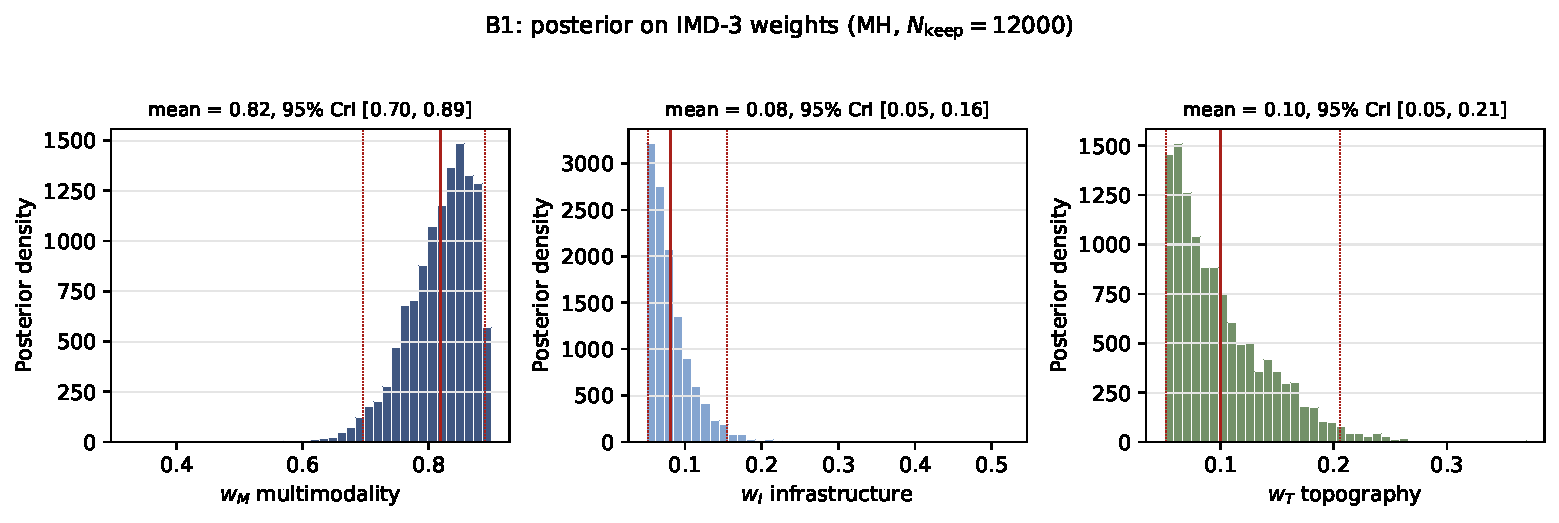
\includegraphics[width=0.98\linewidth]{b1_weights_posterior.pdf}
    \caption{Marginal posterior on the three IMD weights. The
    dashed red lines mark the $2.5$th and $97.5$th percentiles
    of each marginal; the solid red line is the posterior mean.
    Multimodality is credibly the largest weight in $100\,\%$ of
    the $12\,000$ MCMC samples.}
    \label{fig:weights}
\end{figure}

\subsection{Top-of-ranking with credible intervals}
\label{sec:results-ranking}

Propagating the weight posterior to station-level IMDs and
aggregating to city level yields a posterior over city IMDs
that bears a credible interval rather than a single point
(Table~\ref{tab:top10} and Figure~\ref{fig:top10}). Strasbourg
leads the panel with posterior-median IMD $20.5$ (CrI
$[16.0, 30.0]$); Montpellier follows at $18.2$ $[14.3, 27.2]$
and Paris at $17.4$ $[13.6, 26.3]$. The $95\,\%$ credible
intervals of the Top-3 overlap, so the Bayesian framework does
not licence a strict ordering of Strasbourg, Montpellier and
Paris; what it licences is a stable Top-3 \emph{set} that is
clearly separated from the rest of the panel.

\begin{table}[H]
\centering
\caption{Top-10 of the French panel under the Bayesian IMD-3.
The posterior median, $95\,\%$ credible interval, and the
within-city posterior standard deviation are reported.}
\label{tab:top10}
\small
\begin{tabular}{@{}clrcc@{}}
\toprule
Rank & City & Stations & Posterior median IMD &
$95\,\%$ credible interval \\
\midrule
1  & Strasbourg   &  39 & $20.5$ & $[16.0, 30.0]$ \\
2  & Montpellier  &  53 & $18.2$ & $[14.3, 27.2]$ \\
3  & Paris        & 1\,507 & $17.4$ & $[13.6, 26.3]$ \\
4  & Nantes       & 124 & $17.1$ & $[13.4, 25.7]$ \\
5  & Mulhouse     &  60 & $16.5$ & $[12.6, 25.8]$ \\
6  & Caen         &  75 & $14.7$ & $[11.0, 23.7]$ \\
7  & Bordeaux     & 225 & $14.2$ & $[10.2, 23.7]$ \\
8  & Brest        & 115 & $13.6$ & $[10.4, 21.7]$ \\
9  & Rennes       &  57 & $13.5$ & $[9.6,  22.9]$ \\
10 & Dijon        &  40 & $12.9$ & $[9.5,  22.5]$ \\
\bottomrule
\end{tabular}
\end{table}

\begin{figure}[H]
    \centering
    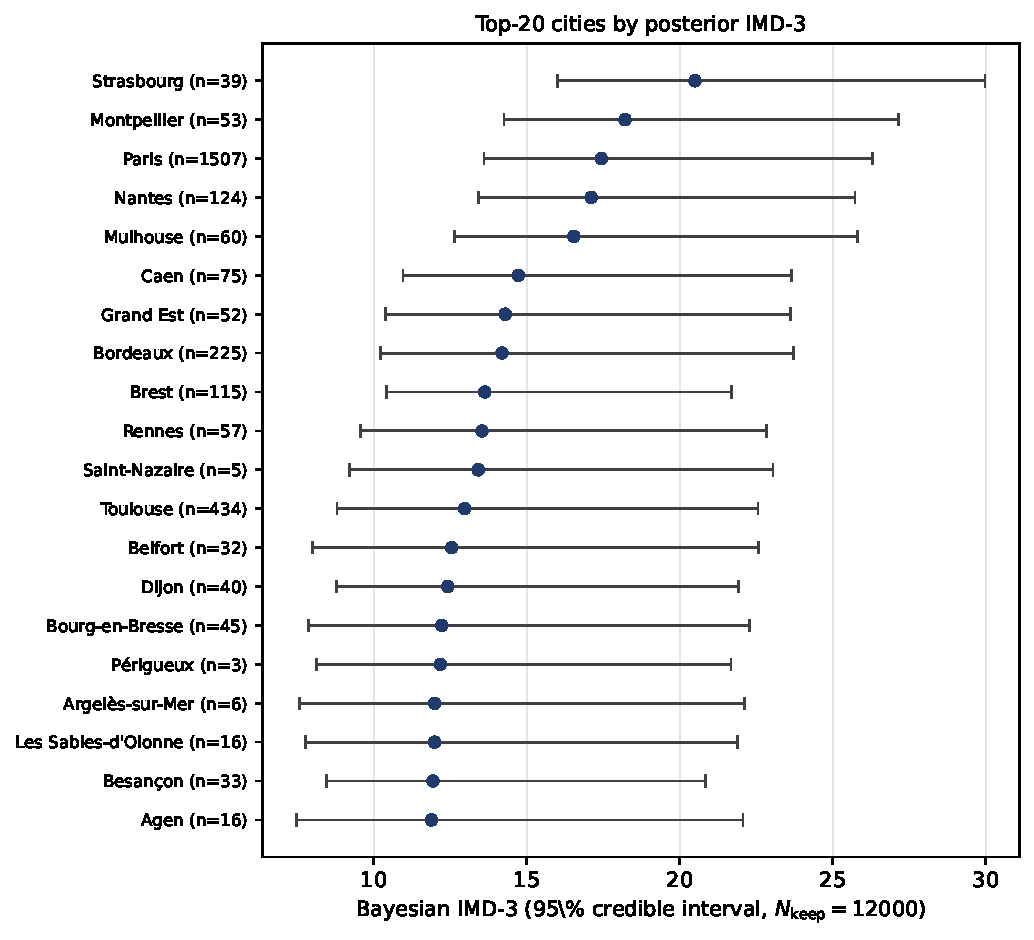
\includegraphics[width=0.78\linewidth]{b1_top_ranking_ci.pdf}
    \caption{Top-20 of the Bayesian IMD-3 with $95\,\%$
    posterior credible intervals. The Top-3 is CI-overlapping
    (Strasbourg, Montpellier, Paris) but clearly separated from
    cities ranked 11th and below.}
    \label{fig:top10}
\end{figure}

\subsection{Within-city station distributions}
\label{sec:results-within}

The Bayesian framework retains the per-station posterior. Each
city is therefore characterised not by a single score but by a
\emph{distribution} of station IMDs whose shape is informative.
Strasbourg's 39 stations span an IMD range of approximately
$15$--$30$; Paris's $1\,507$ stations span a far wider range,
including peripheral stations with IMD comparable to the panel
median (Figure~\ref{fig:within-city}). The within-city station
distribution makes explicit the structural finding that
prior work flagged at the aggregated level: \emph{between-city
ranking is not the only relevant dimension; within-city
heterogeneity is comparable and policy-relevant in its own
right}.

\begin{figure}[H]
    \centering
    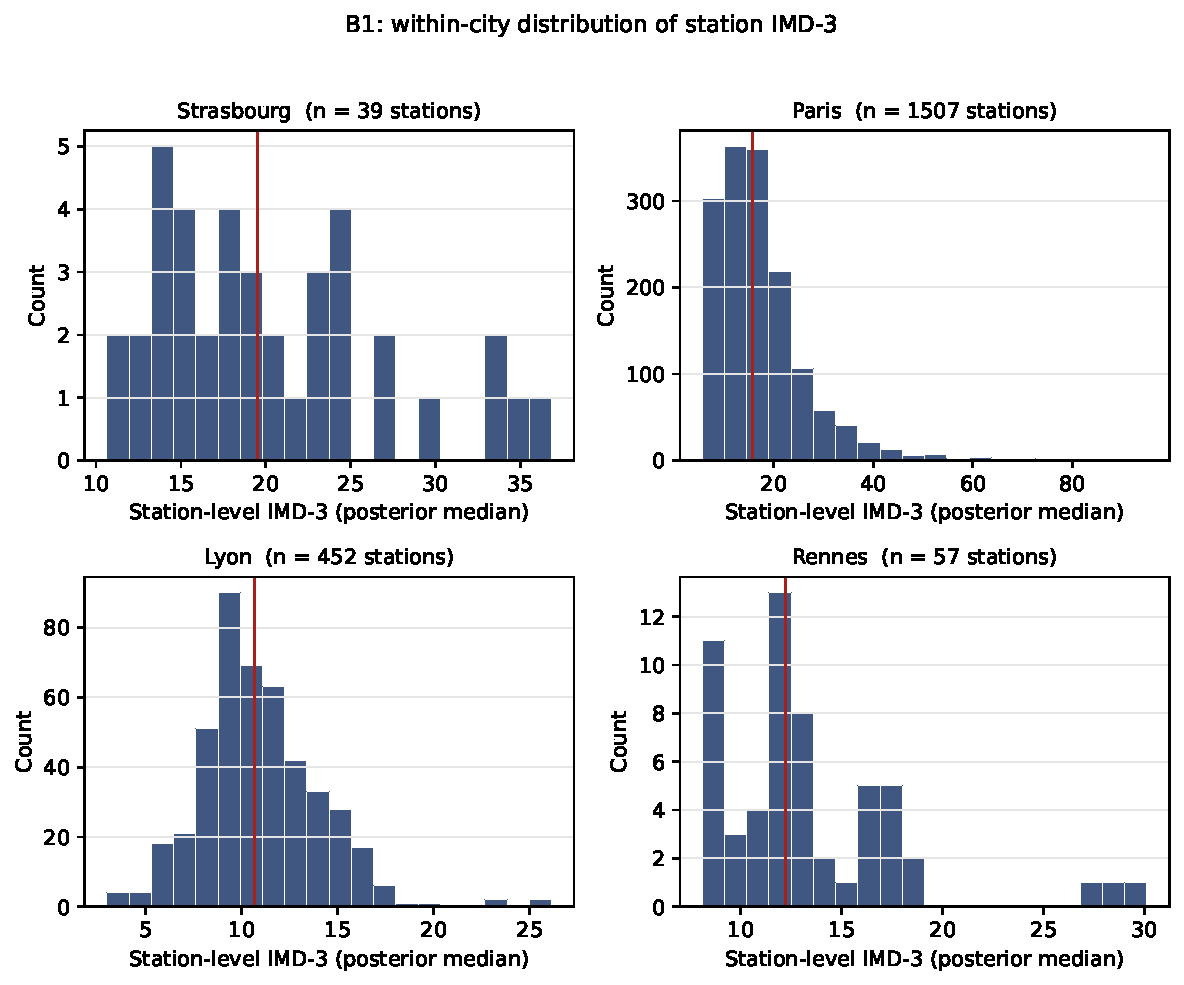
\includegraphics[width=0.95\linewidth]{b1_per_station_distribution_examples.pdf}
    \caption{Within-city distribution of station IMD-3 posterior
    medians for four representative cities. Strasbourg is small
    and dense; Paris is large and heterogeneous; Lyon and Rennes
    fall in between. The vertical red line marks the city
    median.}
    \label{fig:within-city}
\end{figure}

% =========================================================================
\section{Application: priors falsified, equity diagnosed}
\label{sec:application}
% =========================================================================

\subsection{The volumetric prior fails}

A monotone relationship between station count and the IMD
would support the volumetric prior. The empirical relationship
is not monotone. Strasbourg achieves the highest
posterior-median IMD with $39$ stations; Paris ranks third with
$1\,507$ stations; medium-sized cities (Mulhouse, Caen, Brest)
sit between them. The Spearman correlation between station
count and posterior-median IMD on the dock-based panel is
$\rho = +0.18$ ($p = 0.18$). The volumetric metric is therefore
weakly correlated with the IMD and does not predict it
monotonically.

\subsection{The affluence prior fails}

Spearman correlation between the posterior-median IMD and the
median household income per consumption unit on the
dock-based panel is $\rho_{\mathrm{Sp}} = +0.04$ ($p = 0.76$).
We cannot reject the null hypothesis of statistical
independence. The Bayesian framework gives a complementary
formulation: regressing the posterior-median IMD on the
standardised income coefficient yields a posterior mean of
$-0.74$ with a $95\,\%$ credible interval $[-4.76, +3.34]$
that straddles zero. Both formulations falsify the affluence
prior.

\subsection{A spatial-equity index (IES) with credible intervals}

Building on this finding we define a Spatial Equity Index
(IES) as the residual deviation of a city's IMD from its
socio-economic prediction, computed through a Bayesian
Ridge regression with the same conjugate
normal--inverse-gamma framework as our weight calibration.
The four standardised predictors are income per consumption
unit, the Gini index of local income, the share of car-free
households and the share of cycling to work; the regression
returns a posterior on each city's predicted IMD and on the
residual ratio $\IES_i = \IMD_i^{\text{obs}} /
\widehat{\IMD}_i$. Cities with $\IES < 0.85$ in a high
fraction of the posterior draws are flagged as \emph{social
mobility deserts}. We report the prior-invariant
high-confidence shortlist (across $\tau \in \{0.1, 1, 10\}$ for
the regression prior precision) as Amiens, Nancy, Saumur after
the A6 GTFS-completeness patch is applied to Lyon, Marseille
and Lille; the full IES analysis is in the companion repository.

\subsection{The 80\,\% intra-city variance and what it implies}

A one-way ANOVA on the per-station IMD posterior medians
attributes $80.8\,\%$ of the variance to within-city
heterogeneity and $19.2\,\%$ to between-city differences
($\text{ICC}_1 = 0.19$). The Theil--T decomposition gives an
almost identical split ($79.2\,\%$ within, $20.8\,\%$ between).
Under a city-level point-estimate composite, this $80\,\%$
disappears into the city aggregate; under the station-level
Bayesian indicator it is part of the indicator's natural
output. The policy implication is direct: any cycling-environment
intervention designed at city granularity discards the dimension
that carries four-fifths of the variation. Future iterations of
the indicator should operate at sub-municipal granularity (a
$\text{km}^{2}$ grid or a neighbourhood partition).

% =========================================================================
\section{Discussion}
\label{sec:discussion}
% =========================================================================

\subsection{What the Bayesian framing adds}

A Bayesian formulation of a composite indicator yields three
benefits that point-estimate composites do not:

\begin{itemize}
\item \emph{Coherent uncertainty propagation.} The credible
intervals on city IMDs in Table~\ref{tab:top10} are not added
as a separate sensitivity analysis; they emerge from the same
posterior that produced the point estimates. The Bayesian
framework integrates calibration uncertainty, station-sampling
uncertainty and observation noise in a single object.
\item \emph{Identification of effective dimensionality.}
The posterior on $w_M$ at $0.82$ with $P(\text{dominant}) =
1.00$ documents that the IMD is empirically one-dimensional
(plus small refinements), not three-dimensional. Reporting the
indicator as a balanced three-axis composite would have
over-stated the role of infrastructure and topography by
roughly $5\times$ each.
\item \emph{Direct diagnostic of data-quality anomalies.}
A6-affected cities (Lyon, Marseille, Lille) inherit wider
credible intervals when their per-station components carry
documented measurement noise. Point-estimate composites would
have to be re-calibrated to absorb the anomaly; the Bayesian
formulation absorbs it through wider posteriors.
\end{itemize}

\subsection{Policy implications}

Three operational implications follow.

\emph{Use the IMD as a contractual benchmark.}
The composite is computed on data that operators are already
required to publish under the LOM (GBFS station inventories).
Replacing the volumetric default with the IMD in AOM--operator
contracts therefore costs zero marginal data work and reduces
the alignment gap between operator incentives and cyclist
well-being.

\emph{Invest in multimodal integration before fleet expansion.}
The posterior on $w_M$ at $0.82$ identifies multimodality as
the empirically dominant lever. The volumetric counter-example
of Strasbourg ($39$ stations, top of the ranking) versus Paris
($1\,507$ stations, third in the ranking) suggests that the
marginal IMD point per euro of investment is larger for
tramway/metro integration than for fleet expansion -- though
quantifying that statement requires the longitudinal
synthetic-control identification we scope for the next
iteration.

\emph{Operate at station rather than city granularity.}
$80\,\%$ of the IMD variance lives within cities. City-level
targeting of cycling investments discards four-fifths of the
empirical signal. The station-level posteriors output by the
present framework support a direct workflow: rank stations
within each city, identify the worst-served and the
best-served, and recommend specific micro-interventions
accordingly.

\subsection{Limitations and outstanding tests}

The IMD as defined in this paper has four documented
limitations.

\emph{The GBFS snapshot is static.}
The Gold Standard release we consume is a single audited
snapshot; the IMD as published does not reflect the historical
trajectory of a system. A longitudinal synthetic-control test
of the effect of tramway-line openings on the local IMD
trajectory is the dominant outstanding test and is scoped for
the next iteration.

\emph{Safety is reported separately.}
The exposure-confounding documented in the cycling-safety
literature \citep{Reynolds2009, Schepers2014} and the absence
of credible discriminative information in the BAAC layer
support excluding safety from the composite. A clean treatment
requires station-level cyclist exposure data, which is not
currently in the open data catalogue.

\emph{The GTFS layer has documented anomalies.}
Anomaly class A6 affects six panel cities; the present
framework absorbs the anomaly through wider posterior
credible intervals on the affected cities. A cleaner
remediation requires the next Gold Standard release to ingest
both GTFS and OSM heavy-transit tags and take the maximum.

\emph{The panel excludes non-GBFS schemes.}
The IMD covers only systems publishing GBFS, under-representing
end-of-contract operators and community schemes.

% =========================================================================
\section{Conclusion}
\label{sec:conclusion}
% =========================================================================

We have defined the Soft Mobility Index as a three-component
Bayesian composite indicator of cycling-environment quality,
computed at the station level on the audited 46\,139-station
Gold Standard inventory of French bike-sharing systems
\citep{Fosse2026gold}. The Bayesian posterior on the simplex
weights is sharply concentrated on a multimodality-dominated
configuration ($w_M = 0.82$, $95\,\%$ credible interval
$[0.70, 0.89]$, $P(\text{dominant}) = 1.00$): the IMD is
empirically a multimodality index with infrastructure and
topography refinements.

On the 59-city dock-based panel, the indicator falsifies the
volumetric and affluence priors implicit in current policy
communications (Strasbourg with 39 stations leads the ranking;
$\rho(\IMD, \text{income}) = +0.04$, $p = 0.76$) and partitions
the IMD variance into $80\,\%$ within-city and $20\,\%$
between-city. The Bayesian framework propagates the
calibration, sampling and measurement uncertainties into a
single coherent credible interval per station and per city,
naturally absorbs the A6 GTFS-feed completeness anomaly we
document, and supports a workflow that operates at
station rather than city granularity. The four operational
priorities follow: replace the volumetric default by the IMD
in AOM--operator contracts; invest in multimodal integration
before fleet expansion; target stations rather than cities;
and patch the GTFS layer of the Gold Standard pipeline with the
OSM-triangulated multimodality component.

% =========================================================================
\section*{CRediT authorship contribution statement}

\textbf{R. Foss\'e:} Conceptualization, Methodology, Software,
Data curation, Formal analysis, Visualization, Writing -- original
draft, Writing -- review \& editing.
\textbf{G. Pallares:} Conceptualization, Supervision, Funding
acquisition, Writing -- review \& editing.

\section*{Declaration of competing interest}

The authors declare no competing financial interests.

\section*{Data and code availability}

All code, data products, posterior draws and experiment scripts
are released under an open licence at
\url{https://github.com/rohanfosse/bikeshare-data-explorer}.
Reproducible build under
\texttt{papers/03\_imd\_bayesian/}.

% =========================================================================
\bibliography{../references}

\end{document}
